% gc-lab-11-lhopital.tex

\documentclass[11pt]{article}
\usepackage{enumerate}
\usepackage{syllogism} 
\usepackage{october}
\usepackage[table]{xcolor}

\newcounter{aufg}
\setcounter{aufg}{0}
\newcommand{\aufgabe}[0]{\refstepcounter{aufg}\textbf{(\arabic{aufg})}}

\begin{document}

\textbf{Applications of Differential Calculus}

\emph{\CourseName, \CourseNumber}

% solutions are in gc-lab-11-lhopital-solutions.ipynb
% \stackrel{\mbox{LHR}}{=}

% 12
{\aufgabe} Find
\begin{equation}
  \label{eq:eemeeyae}
  \lim_{x\rightarrow{}0^{+}}\sin{}x\ln{}x\notag
\end{equation}

% 11
{\aufgabe} Find
\begin{equation}
  \label{eq:taihahri}
  \lim_{x\rightarrow{}0}\frac{e^{x}-e^{-x}-2x}{x-\sin{}x}\notag
\end{equation}

% \[
% \lim_{x\rightarrow{}0}\frac{e^{x}-e^{-x}-2x}{x-\sin{}x}\stackrel{\mbox{LHR}}{=}\lim_{x\rightarrow{}0}\frac{e^{x}+e^{-x}-2}{1-\cos{}x}\stackrel{\mbox{LHR}}{=}\lim_{x\rightarrow{}0}\frac{e^{x}-e^{-x}}{\sin{}x}\stackrel{\mbox{LHR}}{=}\lim_{x\rightarrow{}0}\frac{e^{x}+e^{-x}}{\cos{}x}=\frac{1+1}{1}=2
% \]

% 2
{\aufgabe} A cylindrical can is to be made to hold one litre of oil.
Find the dimensions that will minimize the cost of the metal to
manufacture the can.

% 1
{\aufgabe} A farmer has 2400ft of fencing and wants to fence off a
rectangular field that borders a straight river. She needs no fence
along the river. What are the dimensions of the field that has the
largest area?

% 10
{\aufgabe} Find
\begin{equation}
  \label{eq:vuciecha}
  \lim_{x\rightarrow{}1}\frac{1-x+\ln{}x}{1+\cos\pi{}x}\notag
\end{equation}

% 6
{\aufgabe} How close does the semi-circle $y=\sqrt{16-x^{2}}$ come to
the point $P=(1,\sqrt{3})$?

\[
f(a)=\sqrt{a^{2}+\left(\sqrt{16-(a+1)^{2}}-\sqrt{3}{\right)^{2}}
  \]

% 7
{\aufgabe} Solve the following equations using Newton's Method. Use a
graphing calculator to get you started.
\begin{equation}
  \label{eq:xeigheuy}
  x^{6}-x^{5}-6x^{4}-x^{2}+x+10=0\notag
\end{equation}
\begin{equation}
  \label{eq:ohtharoh}
  x^{2}(4-x^{2})=\frac{4}{x^{2}+1}\notag
\end{equation}
\begin{equation}
  \label{eq:iejuangi}
  x^{2}\sqrt{2-x-x^{2}}=1\notag
\end{equation}
\begin{equation}
  \label{eq:oungiegu}
  4e^{-x^{2}}\sin{}x=x^{2}-x+1\notag
\end{equation}
\begin{equation}
  \label{eq:ohpaejae}
  3\sin(x^{2})=2x\notag
\end{equation}

% 5
{\aufgabe} For a fish swimming at a speed $v$ relative to the water,
the energy expenditure per unit time is proportional to $v^{3}$. It is
believed that migrating fish try to minimize the total energy required
to swim a fixed distance. If the fish are swimming against a current
$u$ ($u<v$), then the time required to swim a distance $L$ is
$L/(v-u)$ and the total energy $E$ required to swim the distance is
given by
\begin{equation}
  \label{eq:aiyeiyoo}
  E(v)=av^{3}\cdot\frac{L}{v-u}\notag
\end{equation}
where $a$ is the proportionality constant. Determine the value of $v$
that minimizes $E$.

% 4
{\aufgabe} A cone with height $h$ and radius $r$ is inscribed in a
larger cone with height $H$ and radius $R$ so that its vertex is at
the centre of the base of the larger cone. Find $h$ in terms of the
dimensions of the larger cone that makes the volume of the smaller
cone maximal.

\begin{figure}[h]
  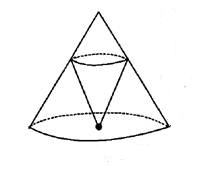
\includegraphics[scale=.75]{./diagrams/coneopt.png}
\end{figure}

% 13
{\aufgabe} Find
\begin{equation}
  \label{eq:gasuchoh}
  \lim_{x\rightarrow{}1}\left(\frac{x}{x-1}-\frac{1}{\ln{}x}\right)\notag
\end{equation}

% 8
{\aufgabe} Of the infinitely many lines that are tangent to the curve
\begin{equation}
  \label{eq:ohtooyiv}
  y=-\sin{}x\notag
\end{equation}
and pass through the origin, there is one that has the largest slope.
Use Newton's Method to find the slope of that line.

% 9
{\aufgabe} Use Newton's Method to find the coordinates of the point on
the parabola
\begin{equation}
  \label{eq:laingiun}
  y=(x-1)^{2}\notag
\end{equation}
that is closest to the origin.

% 3
{\aufgabe} Find the area of the largest rectangle that can be
inscribed in a semicircle of radius $r$.

% \begin{figure}[h]
% 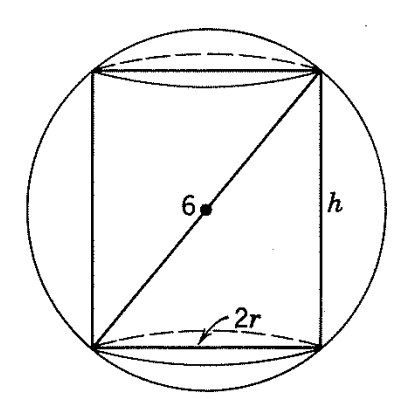
\includegraphics[scale=.4]{./diagrams/cooleyopt.png}
% \end{figure}

\end{document}

